%%% XeLaTeX-article %%%
%# -*- coding: utf-8 -*-
%!TEX encoding = UTF-8 Unicode
%!TEX TS-program = xelatex  
%---------------------虽然加了%还是要保留!

\documentclass[17pt]{beamer}
\mode<presentation>
{
\usetheme[width=40pt]{Hannover}
\usecolortheme[]{dove}
\usefonttheme[]{structurebold}
\setbeameroption{hide notes}
}

\usepackage{fontspec}
\setmainfont{Arial} %设置主字体
\newfontfamily\sanskritfont[Script=Devanagari,Mapping=romantodevanagari,Scale=1.15]{Sanskrit 2003}             %输出天城体
%\newfontfamily\sanskritfont[Mapping=tex-text]{Times New Roman}              %输出转写
\doublehyphendemerits=-10000
\newcommand{\skt}[1]{{\sanskritfont{#1}}} %输出天城体
\newcommand{\skttrans}[1]{{\skt{#1}~#1}}  %输出天城体和转写
%----------------------------------------------------设置梵文输入方法 danda । ॥

\usepackage[UTF8,fontset=windows]{ctex}
\usepackage{amsmath}
%----------------------------------------------------设置中文环境

\usepackage{graphicx}
\usepackage{flafter} 
\graphicspath{{pic/}}
\usepackage{booktabs} 
%-----------------------------------------插图表格

\usepackage{hyperref} 
\usepackage{xcolor}
%------------------------------颜色

\newcommand{\verbroot}[1]{{$\sqrt{#1}$}}
\newcommand{\sktroot}[1]{{\verbroot{}\skt{#1}}}
\newcommand{\skttransroot}[1]{{\sktroot{#1}~#1}}
%---------------------------------------------------------------词根

\title{{梵语入门}}
\subtitle{6. 元音转换}
\author[张雪杉]{文学院~~张雪杉 \\ zhangxueshan@sdnu.edu.cn}
\date{}
%\institute{}



\begin{document}	


\begin{frame}
  \titlepage
\end{frame}

\begin{frame}
  \frametitle{本节内容}
  \tableofcontents
\end{frame}

\section{上节作业}

\begin{frame}{第六章练习4}
  \small
  \raggedright
  \begin{verse}
    \skt{1) īśvarasya gṛhaṃ viśāmaḥ ।}   \\
    \skt{2) bālaḥ īśvarasya gṛhe kiṃ karoti ।}   \\
    \skt{3) bālau aśvābhyāṃ saha vanaṃ viśataḥ।}   \\
    \mbox{\skt{4) bālāḥ puruṣasya vacanāni bodhanti hṛṣyanti ca ।}}  \\
    \skt{5) īśvara kim icchasi ।}   \\
    \skt{6) bālaḥ devasya guṇān smarati ।}   \\
    \skt{7) śūrau yuddhāt mitraṃ bharataḥ ।}   \\
    \skt{8) devaḥ atra vane iti bālaḥ bodhati ।}   \\
    \skt{9) nṛpāya janāḥ bālāḥ iva priyāḥ ।}   \\
  \end{verse}
\end{frame}  

\begin{frame}{第六章练习4}
  \small
  \begin{verse}
    \mbox{\skt{10) api bālasya mitrāṇi śūrāṇi pāpāni vā ।}}  \\
    \mbox{\skt{11) aśvaḥ naraṃ bālau ca vanāt nagaraṃ prati bharati ।}}  \\
    \skt{12) śūrāḥ narāḥ api siṃhau vane paśyatha ।}   \\
    \skt{13) bālaḥ mitrasya vacanāni na smarati ।}   \\
    \mbox{\skt{14) aśvāḥ yuddhāt hṛṣyanti iti śūraḥ bodhati ।}} \\
    \skt{15) api naraḥ aśvaḥ ca vyāghrān paśyataḥ ।}   \\
    \skt{16) īśvarāḥ pāpānāṃ narāṇām aśvān haranti gṛhān ca lumpanti ।}   \\
    \skt{17) vṛkṣe eva phalāni paśyāmi ।}   \\
    \mbox{\skt{18) iha yuddhe pāpān śūrān ca janān paśyāmi ।}}   \\
  \end{verse}
\end{frame}  
 

\section{元音转换}
\begin{frame}{\insertsection }
    \tableofcontents[currentsection]
\end{frame}

\begin{frame}{\insertsection }
    \centering    
    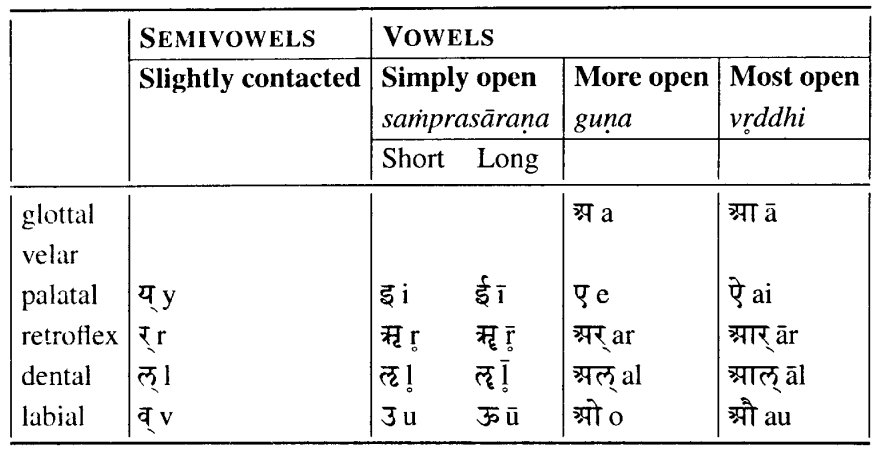
\includegraphics[width=\textwidth]{gunavrddhi.png}
\end{frame}

\begin{frame}{\insertsection ~~\insertsubsection}
  \begin{itemize}
    \item 按照名词变化的词:
    
    名词、代词、形容词、分词
  \end{itemize}
\end{frame}

\begin{frame}{\insertsection ~~相关概念}
  \begin{itemize}
    \item 形态层面:
    
    词干(语干、词基)、词尾(格尾)
    \item 意义层面:
      
    性、数、格
  \end{itemize}
\end{frame}

\subsection{性和数}
\begin{frame}{\insertsubsection}
  \begin{itemize}
    \item
      词性:
      
      阳性、阴性、中性
    \item
      数:
      
      单数、双数、复数
  \end{itemize}  
\end{frame}

\subsection{格的意义}
\begin{frame}{\insertsubsection}
  \small
  \centering
  \begin{tabular}{@{}llllll@{}} % 6 columns
    次序 & 格 & 英文名 & 意义  \\
    1 & 主格 & Nominative & 主语  \\
     & 呼格 & Vocative & 呼语  \\
    2 & 业格 & Accusative & 直接宾语、方向 \\
    3 & 具格 & Instrumental & 工具、伴随  \\
    4 & 为格 & Dative & 间接宾语  \\
    5 & 从格 & Ablative & 来源、理由  \\  
    6 & 属格 & Genitive & 所有格、关系  \\
    7 & 依格 & Locative & 位置、时间  \\ 
  \end{tabular}
\end{frame}

\subsection[a的变格]{以a结尾的名词变格}
\begin{frame}{\insertsubsection ~~阳性}
  \small
  \centering
  \resizebox{\textwidth}{!}{
    \begin{tabular}{@{}llllll@{}} % 6 columns
      格 & 单数 & 双数 & 复数  \\
      主 & \skttrans{devaḥ}  & \skttrans{devau} & \skttrans{devāḥ}   \\
      呼 & \skttrans{deva} & \skttrans{devau} & \skttrans{devāḥ} \\
      业 & \skttrans{devam} & \skttrans{devau} & \skttrans{devān} \\
      具 & \skttrans{devena} & \skttrans{devābhyām} & \skttrans{devaiḥ} \\
      为 & \skttrans{devāya} & \skttrans{devābhyām} & \skttrans{devebhyaḥ} \\
      从 & \skttrans{devāt} & \skttrans{devābhyām} & \skttrans{devebhyaḥ} \\
      属 & \skttrans{devasya} & \skttrans{devayoḥ} & \skttrans{devānām} \\
      依 & \skttrans{deve} & \skttrans{devayoḥ} & \skttrans{deveṣu} \\
    \end{tabular}
  }
\end{frame}

\begin{frame}{\insertsubsection ~~中性}
  \small
  \centering
  \resizebox{\textwidth}{!}{
    \begin{tabular}{@{}llllll@{}} % 6 columns
      格 & 单数 & 双数 & 复数  \\
      主 & \skttrans{vanam} & \skttrans{vane} & \skttrans{vanāni} \\
      呼 & \skttrans{vana} & \skttrans{vane} & \skttrans{vanāni} \\
      业 & \skttrans{vanam} & \skttrans{vane} & \skttrans{vanāni} \\
      具 & \skttrans{vanena} & \skttrans{vanābhyām} & \skttrans{vanaiḥ} \\
       & 下同 &  &  \\
    \end{tabular}
  }
  \begin{itemize}
    \item 形容词根据其修饰的名词变化。
    \item 阴性名词有的以ā结尾,有的以ī结尾。
  \end{itemize}
\end{frame}



\section{连声}
\begin{frame}{\insertsection }
    \tableofcontents[currentsection]
\end{frame}

\begin{frame}{\insertsection ~~分类}
  \begin{itemize}
    \item 词间连声
    \item 词内连声
  \end{itemize}
\end{frame}

\subsection{n的顶化}

\begin{frame}{\insertsubsection  ~~条件 }
  \begin{enumerate}
    \item
      肯定条件:
      
      词内n前有r, ṛ, ṝ或ṣ。
    \item
      肯定条件:
      
      n后是n, m, y, v或者元音。
    \item
      否定条件:
      
      r, ṛ, ṝ或ṣ和n之间有齿音、腭音、顶音或者s和ś。
  \end{enumerate}
\end{frame}

\begin{frame}{\insertsubsection  ~~例子 }
  %\small
  \centering
  \begin{tabular}{@{}lllll@{}} % 7 columns: type, length/type, and 5 vowels
    条件 & 顶化 & 不顶化 \\[0.2cm]
    1  & \skt{mitreṇa}~mit\textcolor{red}{r}eṇa  & \skttrans{vanena}  \\
    2  & \skt{brahmaṇā}~brahmaṇ\textcolor{red}{ā} & \skttrans{brahman} \\
    3  & \skttrans{rāmeṇa} & \skt{rathena}~ra\textcolor{red}{th}ena  \\
  \end{tabular} 
\end{frame}

\section{本节作业}

\begin{frame}{\insertsection }
  \begin{itemize}
    \item
      自学第六章iti的说明
    \item
      第六章练习4
    \item
      阅读教材第5\nobreakdash-6课相关内容
    \bigskip
    \item
      现在请做学习通\nobreakdash-章节\nobreakdash-课后问卷
  \end{itemize}
\end{frame}  

\end{document}	
